% !TeX program = xelatex
% !BIB program = bibtex
% !TeX encoding = UTF-8
\documentclass[preprint,12pt]{elsarticle}

\ifdefined\synctex
  \synctex=1
\fi

\usepackage{ctex}
\usepackage{amssymb}
\usepackage{amsmath}
\usepackage{graphicx}
\usepackage{booktabs}
\usepackage{geometry}
\usepackage{hyperref}
\usepackage{subcaption}
\usepackage{caption}
\usepackage{float}
\usepackage{algorithm}
\usepackage{algpseudocode}
\usepackage{multirow}
\usepackage{array}
\usepackage{enumitem}

\graphicspath{{./figures/}}
\journal{Engineering Applications of Artificial Intelligence}

\renewcommand{\algorithmicrequire}{\textbf{Require:}}
\renewcommand{\algorithmicensure}{\textbf{Ensure:}}

\begin{document}

\begin{frontmatter}

\title{Reinforcement Learning-Based Computer Numerical Control Motion Planning with Learnable Preview Distance and Jerk-Constrained Action Projection}

\author[1]{作者姓名}
\affiliation[1]{organization={某某大学/机构},
            addressline={某某路},
            city={某某市},
            postcode={000000},
            country={中国}}

\begin{abstract}
Computer numerical control (CNC) machining requires motion planning that smooths mixed tool paths within a contour tolerance band while preserving feed efficiency and satisfying velocity, acceleration, and jerk limits. This paper proposes a structured reinforcement learning (RL) decision framework for tolerance-band CNC motion planning, where Proximal Policy Optimization (PPO) learns steering, feedrate, and preview-distance actions so that the policy can actively select the geometric perception scale needed by straight, corner-entry, corner-passing, and corner-exit phases. An interpretable kinematic constraint module (KCM) is embedded as a jerk-constrained action-projection layer, transforming unconstrained policy intentions into interpolation commands that satisfy linear and angular velocity, acceleration, and jerk bounds. Experiments on square, circular, and butterfly paths show that the proposed method generates tolerance-feasible smoothed trajectories and eliminates the jerk violations observed in a neural network controller (NNC) baseline, improving the dynamic executability of CNC motion planning under complex geometric changes.
\end{abstract}

\begin{keyword}
computer numerical control \sep reinforcement learning \sep learnable preview distance \sep jerk-constrained action projection
\end{keyword}

\end{frontmatter}

\section{引言}
\label{sec:intro}

在高速高精度加工中，CAM 输出的刀具路径通常由长短不一的离散直线段和圆弧段构成。程序段交接处的切向和曲率不连续，会带来几何连续性和运动学可执行性问题，导致机床为保持轮廓精度而在拐角区域频繁降速；直接高速通过又会带来较大的加速度、捷度和轮廓误差。数控运动规划要解决的直接问题，就是将 CAM 生成的离散刀具路径转换为满足轮廓允差、速度、加速度和捷度约束的可执行插补轨迹。因此，运动规划是决定加工质量和加工效率的关键环节。

传统数控运动规划通常采用先轨迹平滑、再速度规划的串行流程。轨迹平滑方法用于改善离散程序段之间的几何连续性，其中局部轨迹平滑方法通过构造连续过渡曲线改善相邻程序段连接，例如 Li 等人\cite{Li2023}针对直线/圆弧混合刀具路径提出运动重叠方法，通过相邻运动段之间的重叠过渡改善混合路径连接连续性；Zhao 等人\cite{Zhao2013}利用曲率连续 B 样条过渡实现短线段的实时前瞻插补，提高了拐角过渡的几何连续性。全局方法在全局范围内重构离散路径，例如 Song 等人\cite{Song2021}将控制点分配与 FIR 滤波结合，用于连续短线段刀具路径的全局平滑；Sun 等人\cite{Sun2024}面向五轴加工路径研究平滑插补方法，以提高复杂路径下的插补效率。速度规划方法则在给定几何轨迹上生成进给曲线，例如 Lee 等人\cite{Lee2011}研究 NURBS 插补中的进给率调度；Erkorkmaz 和 Altintas\cite{Erkorkmaz2001}通过捷度受限轨迹生成与五次样条插补改善高速 CNC 加工过程中的动态平稳性；Song 等人\cite{Song2020}利用前瞻窗口和轴驱动约束进行长五轴样条路径的自适应进给率规划。

串行式流程清晰、便于实现。已有研究表明，在先轨迹平滑、再速度规划的流程下，速度规划效果受到已生成几何轨迹的限制\cite{Zhang2021}；在捷度约束和非平稳边界条件下，后续速度规划主要是在既定轨迹上提高动态可执行性\cite{Zhang2026,WangAIM2025}。因此，几何轨迹一旦确定，后续速度规划主要只能沿既定轨迹调整进给速度，难以进一步改变拐角区的实际执行路径。与此同时，前瞻窗口和动态前瞻相关研究表明，前方几何信息的利用方式会影响速度规划和局部几何响应，固定前瞻范围难以同时适配直线进给、接近拐角、通过拐角和离开拐角等路径的不同阶段\cite{Song2020,Zhong2025}。因此，需要构建统一的闭环决策式运动规划方法，使控制器能够同时完成允差带内的轨迹规划和受运动学约束的进给速度生成。

为解决这一问题，研究者开始尝试用学习型策略根据当前刀具路径、前方几何信息和运动状态直接生成插补控制动作。Li 等人较早将强化学习用于 CNC 轨迹平滑，提出 neural-network numerical control（NNC）直接轨迹平滑方法\cite{Li2020}。该方法将轨迹平滑转化为动作决策问题，神经网络根据当前刀具路径和运行状态，在每个插补周期直接输出伺服控制命令，其动作由角度变化和步长变化构成，并进一步转化为位置命令，奖励主要由当前点到 G-code 路径的轮廓误差定义。实验结果表明，NNC 相比局部平滑方法具有更高加工效率，相比全局平滑方法具有更好的轮廓精度。除 NNC 外，Samsonov 等人利用深度表征学习和强化学习研究 CNC 制造决策问题\cite{Samsonov2023}；Alizadeh Kolagar 等人将深度强化学习与捷度有界轨迹生成器结合，用于提高学习控制过程中的运动学可执行性\cite{Alizadeh2025}。在安全学习控制领域，Pham 等人的 OptLayer\cite{Pham2018}、Alshiekh 等人的 shielding\cite{Alshiekh2018}、Cheng 等人的 control-barrier-function 安全控制\cite{Cheng2019}以及 Wabersich 和 Zeilinger 的 predictive safety filter\cite{Wabersich2021}也表明，学习动作通常需要通过投影或过滤机制满足外部约束。

上述 NNC 方法仍有两个需要进一步处理的问题：一是神经网络动作直接转化为插补位置或伺服命令，速度、加速度和捷度约束缺少显式约束处理或执行层投影机制，策略输出可能超出机床运动学边界；二是奖励主要围绕轮廓误差构造，对路径进度、方向一致性、运动平滑性和拐角阶段差异的设计不足，策略在尖角或曲率快速变化区域难以主动利用允差带选择更平滑的过渡轨迹。

为此，本文提出一种基于可学习前瞻与捷度约束动作投影的强化学习数控运动规划方法。为区别于直接神经控制方法（NNC），本文将该框架称为 J-NNC（Jerk-constrained Neural Numerical Controller）。本文将混合路径运动规划建模为允差带内的受约束序列决策问题，使策略在同一闭环中输出转向、进给与前瞻距离调节动作；同时，在状态构造中引入拐角信息和多尺度前方几何信息，在奖励中联合考虑路径进度、轮廓误差、方向一致性和运动平滑性，并由运动学约束模块（kinematic constraint module, KCM）将约束前控制量投影为满足速度、加速度与捷度约束的插补控制量。传统串行式运动规划框架与 J-NNC 闭环运动规划框架的差异如图~\ref{fig:comparison_arch}所示。本文的主要贡献如下：

\begin{enumerate}
  \item 将实时运动学状态、轮廓误差、拐角信息和多尺度前方几何信息统一为策略输入，并将前瞻距离作为可学习动作，使策略能够根据不同几何阶段调节感知尺度，在允差带内形成更平滑的局部过渡轨迹。

  \item 在策略输出与执行之间引入 KCM 运动学约束模块，将策略给出的转向和进给转换为满足速度、加速度和捷度边界的执行控制量，提高学习策略输出的运动学可执行性。

  \item 在 square、circle 和 butterfly 三类代表性路径上进行对比实验和消融实验，结果表明 J-NNC 均达到成功终止，最终路径进度均为 $1.000$，线捷度最大相对超限为 $0$；与 NNC 基线和无 KCM 消融配置相比，本文方法能够在保持路径推进的同时避免捷度超限。
\end{enumerate}

\begin{figure}[htbp]
    \centering
    
\includegraphics[width=0.9\linewidth]{fig1.pdf}
    \caption{传统串行式运动规划与 J-NNC 运动规划框架对比。J-NNC 表示 Jerk-constrained Neural Numerical Controller，即带捷度约束动作投影的神经网络数控运动规划器。}
    \label{fig:comparison_arch}
\end{figure}

本文余下内容安排如下：第二章给出问题定义与约束建模；第三章介绍所提出的方法；第四章给出实验设置、评价指标与结果分析；第五章给出局限性分析与未来展望。

\section{问题定义与约束建模}
\label{sec:problem}

本章给出与本文方法直接相关的任务定义、几何约束与执行约束，为后续方法部分提供必要的形式化基础。

\subsection{刀具路径与几何可行域}
给定由CAM系统生成的离散刀位点序列
\begin{equation}
P_{raw}=\{p_1,p_2,\dots,p_N\},
\end{equation}
其中 $p_i\in\mathbb{R}^2$ 表示插补平面内的参考点。设轮廓允差为 $\varepsilon$，则参考路径两侧各偏置 $\varepsilon/2$ 后可得到一条允许策略局部偏离的几何可行域：
\begin{equation}
\Omega=\{x\mid d(x,P_{raw})\leq \varepsilon/2\},
\label{eq:feasible_region}
\end{equation}
式中 $d(x,P_{raw})$ 为点 $x$ 到参考路径的最小距离。该定义意味着允许策略在允差带内进行局部几何重分配，以换取更平滑的拐角通过过程,不是严格贴近原始轨迹。

\begin{figure}[htbp]
    \centering
    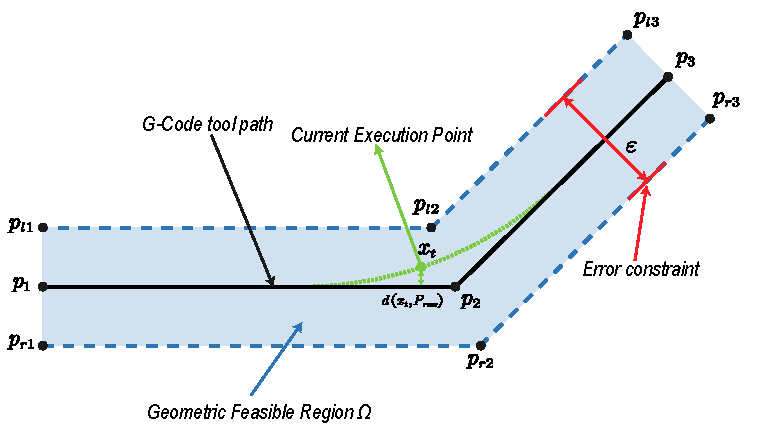
\includegraphics[width=0.9\linewidth]{fig2.pdf}
    \caption{参考路径与轮廓允差带构成的几何可行域。}
    \label{fig:feasible_region}
\end{figure}

为便于在闭环决策中感知局部几何，我们进一步对参考路径进行弧长参数化，并在当前投影弧长 $\ell_t$ 附近提取法向误差、切向方向、到下一拐角距离以及下一拐角转角等量。这些量既参与状态构造，也参与奖励加权与拐角模式判定。

\subsection{受约束动作决策表述}
在每个插补周期 $\Delta t$ 内，策略接收当前状态 $s_t$ 并输出归一化动作 $a_t^{\pi}$。运动学约束模块（kinematic constraint module, KCM）输出的执行控制量作用于环境后，环境更新位置、姿态及运动学状态，并返回即时奖励 $r_t$。因此，本文任务可以写成一个受约束的序列决策问题：
\begin{equation}
\max_{\pi}\ \mathbb{E}_{\pi}\left[\sum_{t=0}^{T} \gamma^t r_t\right],
\end{equation}
同时满足几何约束
\begin{equation}
x_t\in \Omega,
\end{equation}
以及执行侧运动学约束
\begin{equation}
|v_t|\leq V_{\max},\quad |a_t|\leq A_{\max},\quad |j_t|\leq J_{\max},
\end{equation}
\begin{equation}
|\omega_t|\leq \Omega_{\max},\quad |\dot{\omega}_t|\leq A^{\omega}_{\max},\quad |\ddot{\omega}_t|\leq J^{\omega}_{\max}.
\end{equation}
其中 $v_t,a_t,j_t$ 分别表示线速度、线加速度与线捷度，$\omega_t,\dot{\omega}_t,\ddot{\omega}_t$ 分别表示角速度、角加速度与角捷度。

\section{方法}
\label{sec:method}

\subsection{总体框架}
本文将混合刀具路径运动规划表述为强化学习框架下的闭环决策过程。该过程中，策略网络作为智能体，带有轮廓允差和运动学约束的刀具路径仿真系统作为环境。在每个插补周期内，环境根据当前执行位置、运动学状态、局部拐角信息和前方几何信息构造状态 $s_t$；策略 $\pi_\theta$ 根据 $s_t$ 输出动作 $a_t$，用于描述当前周期的转向、进给和前瞻距离调节意图；动作经 KCM 修正后作用于环境，环境更新到下一状态 $s_{t+1}$，并根据路径进度、轮廓误差和运动平滑性返回奖励 $r_t$。训练阶段通过奖励反馈更新策略参数，使策略逐步学习在允差带内完成轨迹平滑、速度规划和运动学约束满足的控制规律。

本文方法的总体框架如图~\ref{fig:framework}所示。给定参考路径与轮廓允差，系统首先在环境侧完成路径投影、拐角扫描与前瞻几何提取，构造当前时刻的结构化状态向量；随后，策略网络输出归一化动作，其中转向分量与进给分量被映射为约束前运动控制量 $(\omega^{pre}_t, v^{pre}_t)$，前瞻分量被映射为当前前瞻距离 $L_t$；最后，KCM 根据上一时刻的速度、加速度和捷度状态，对 $(\omega^{pre}_t, v^{pre}_t)$ 进行在线约束投影，得到满足速度、加速度与捷度限制的执行控制量 $(\omega_t, v_t)$。执行结果反过来更新当前位置、运动学量、拐角相位与前瞻观测，并在训练阶段通过奖励信号参与策略更新，形成完整的强化学习运动规划闭环。

\begin{figure}[htbp]
    \centering
    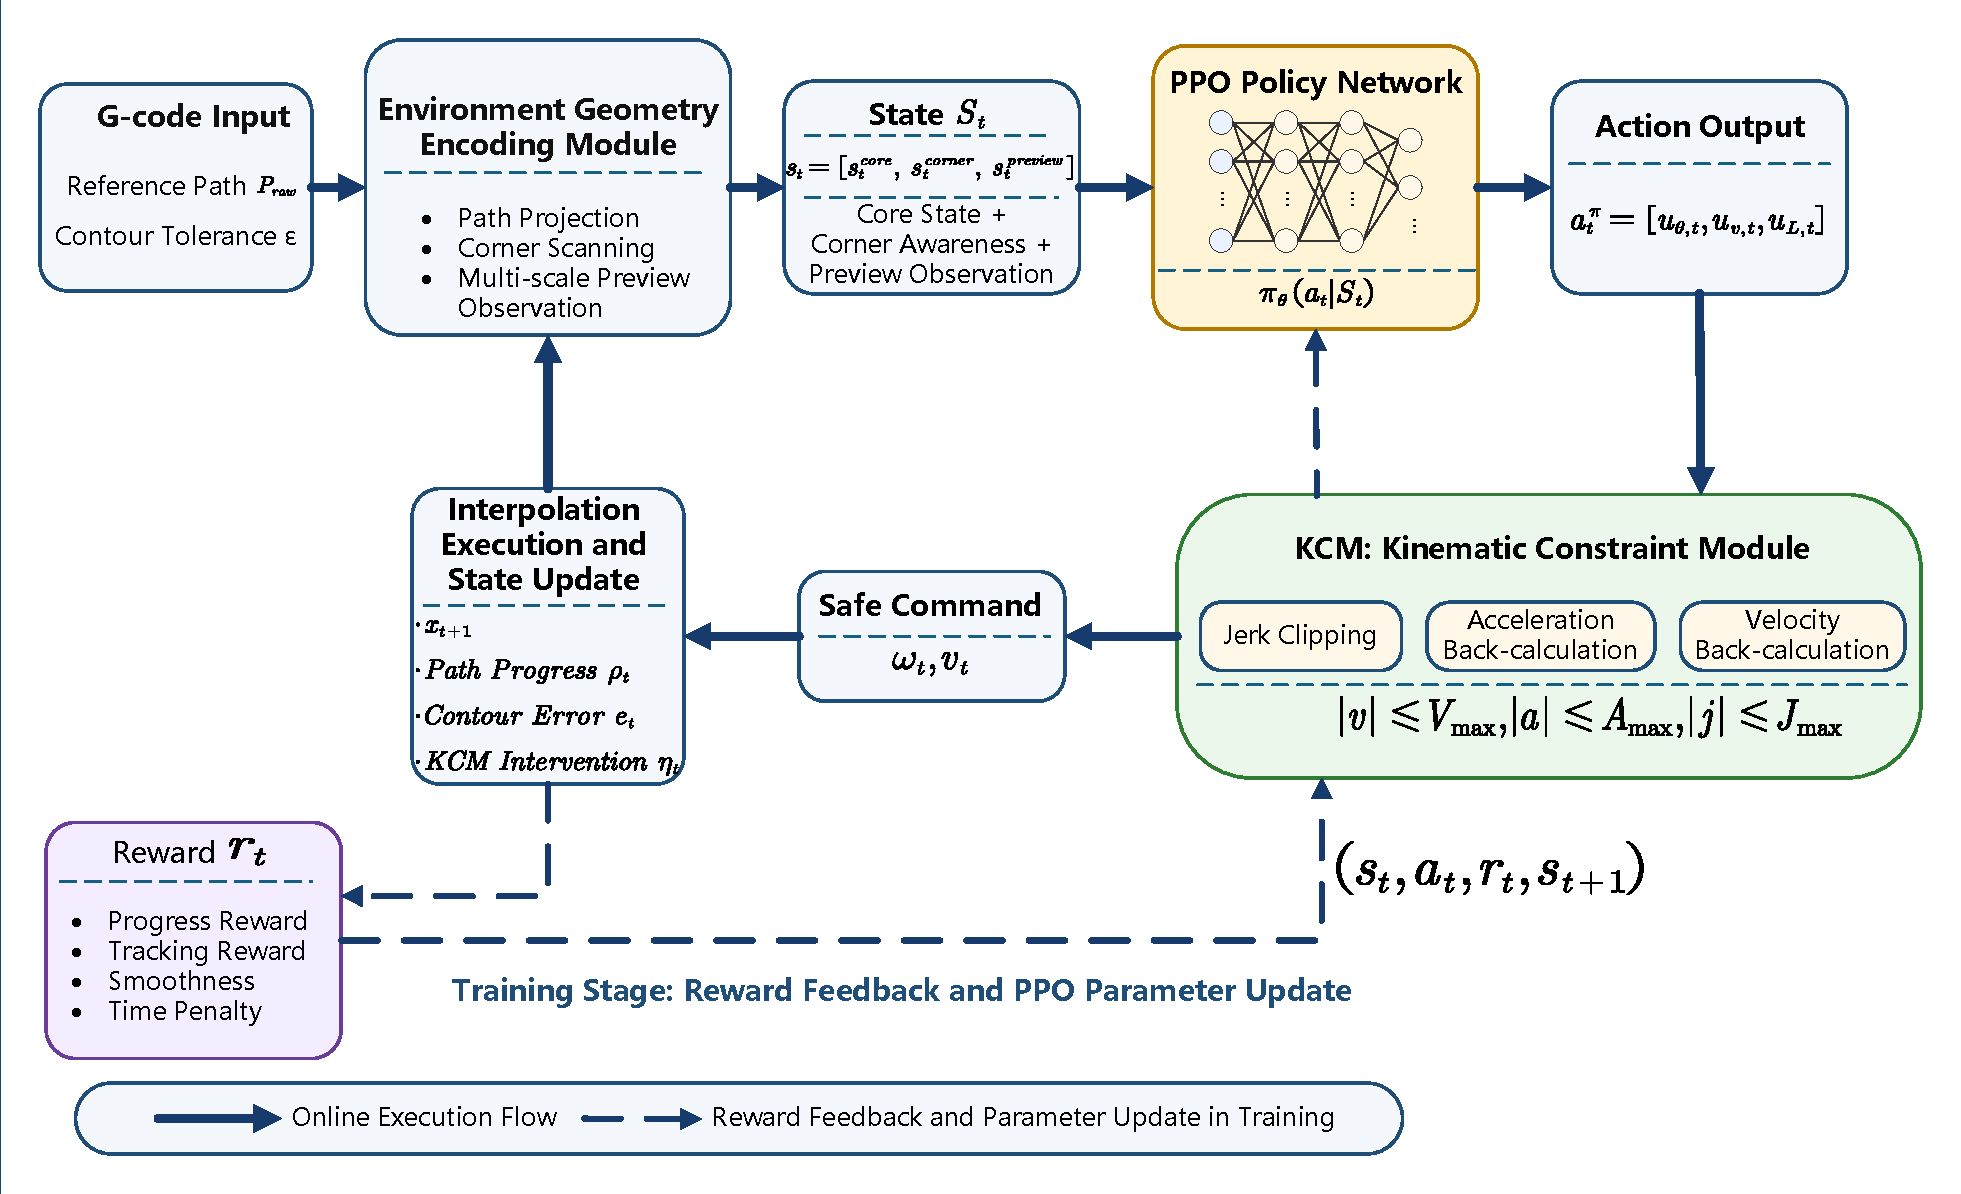
\includegraphics[width=0.9\linewidth]{fig3.pdf}
    \caption{本文方法的总体闭环框架。}
    \label{fig:framework}
\end{figure}

\subsection{状态设计}
本文采用一种分层的结构化状态表示：
\begin{equation}
s_t=[s_t^{core},\ s_t^{corner},\ s_t^{preview}].
\end{equation}
其中 $s_t^{core}$ 描述当前时刻的局部跟踪与运动学状态，$s_t^{corner}$ 描述当前路径段与下一拐角之间的关系，$s_t^{preview}$ 描述前方若干距离处的几何变化趋势。

\paragraph{(1) 核心状态 $s_t^{core}$} 核心状态采用8维构造：
\begin{equation}
s_t^{core}=[\bar e_t,\ \bar e_{n,t},\ \bar\tau_t,\ \bar v_t,\ \bar a_t,\ \bar\omega_t,\ \rho_t,\ \bar d_{c,t}],
\end{equation}
其中 $\bar e_t$ 为归一化轮廓误差，$\bar e_{n,t}$ 为带符号法向误差，$\bar\tau_t$ 为当前航向与局部切向方向之间的归一化夹角误差，$\bar v_t$、$\bar a_t$、$\bar\omega_t$ 分别为归一化线速度、线加速度和角速度，$\rho_t\in[0,1]$ 为路径整体进度，$\bar d_{c,t}$ 为到下一拐角距离的归一化量。

\paragraph{(2) 拐角感知状态 $s_t^{corner}$} 拐角感知状态构造为4维特征：
\begin{equation}
s_t^{corner}=[\bar\phi_t,\ \sigma_t,\ m_t,\ \sigma_t\bar e_{n,t}],
\end{equation}
其中 $\bar\phi_t$ 为下一拐角转角的归一化值，$\sigma_t\in\{-1,0,1\}$ 表示拐角转向符号，$m_t\in\{0,1\}$ 表示是否处于拐角影响区间，$\sigma_t\bar e_{n,t}$ 则给出了相对于转向内侧或外侧的带符号位置关系。

\paragraph{(3) 前瞻观测 $s_t^{preview}$} 本文沿参考路径弧长方向设置若干前瞻尺度 $\{\lambda_k\}_{k=1}^{N_L}$。记当前执行点在参考路径上的投影弧长坐标为 $\ell_t$，第 $k$ 个前瞻尺度对应的前方观测点定义为
\begin{equation}
q_t^{(k)}=P_{raw}(\ell_t+\lambda_k L_t),\qquad k=1,\dots,N_L,
\end{equation}
其中 $\lambda_k$ 为尺度系数，$L_t$ 为当前周期采用的基础前瞻距离。由此，近、中、远前瞻点均沿参考路径弧长方向确定，而不是由当前执行方向上的射线交点确定。随后在每个尺度上提取前方观测点相对于当前切向的角度变化和距离比例：
\begin{equation}
s_t^{preview}=\big[\Delta \theta_t^{(1)},\ \bar d_t^{(1)},\ \dots,\ \Delta \theta_t^{(N_L)},\ \bar d_t^{(N_L)}\big].
\end{equation}
其中 $\Delta \theta_t^{(k)}$ 表征第 $k$ 个前瞻尺度上的方向变化趋势，$\bar d_t^{(k)}$ 表征当前位置到该前瞻点的归一化距离。当前实现中，主配置采用3个前瞻尺度。

\subsection{动作空间与运动学约束模块}
策略网络在每个周期输出归一化动作
\begin{equation}
 a_t^{\pi}=[u_{\theta,t},u_{v,t},u_{L,t}],
\end{equation}
其中 $u_{\theta,t}\in[-1,1]$ 表示转向控制的归一化动作分量，$u_{v,t}\in[0,1]$ 表示进给控制的归一化动作分量，$u_{L,t}\in[0,1]$ 表示前瞻距离调节分量。设前瞻距离允许范围为 $[L_{\min},L_{\max}]$，则其物理量映射为
\begin{equation}
L_t=L_{\min}+u_{L,t}(L_{\max}-L_{\min}).
\end{equation}
策略输出首先被映射为物理空间中的约束前运动控制量：
\begin{equation}
\omega_t^{pre}=u_{\theta,t}\Omega_{\max},\qquad v_t^{pre}=u_{v,t}V_{\max}.
\end{equation}
前瞻距离 $L_t$ 直接参与局部参考方向与前瞻几何的计算。随后，KCM 根据上一时刻运动学状态对 $(\omega_t^{pre},v_t^{pre})$ 进行约束投影。以线速度通道为例，设上一周期的线速度和线加速度分别为 $v_{t-1}$ 与 $a_{t-1}$，则有
\begin{equation}
 a_t^{pre}=\frac{v_t^{pre}-v_{t-1}}{\Delta t},
\end{equation}
\begin{equation}
 j_t^{pre}=\frac{a_t^{pre}-a_{t-1}}{\Delta t}.
\end{equation}
KCM 首先对约束前捷度进行裁剪：
\begin{equation}
 j_t=\mathrm{clip}(j_t^{pre},-J_{\max},J_{\max}),
\end{equation}
再由此反算本周期可实现的加速度与速度：
\begin{equation}
 a_t=\mathrm{clip}(a_{t-1}+j_t\Delta t,-A_{\max},A_{\max}),
\end{equation}
\begin{equation}
 v_t=\mathrm{clip}\left(v_{t-1}+a_{t-1}\Delta t+\frac{1}{2}j_t\Delta t^2,0,V_{\max}\right).
\end{equation}
角速度通道采用完全相同的约束流程。得到的 $(\omega_t,v_t)$ 作为环境执行控制量。

本文还定义 KCM 干预度：
\begin{equation}
\eta_t=\frac{|v_t-v_t^{pre}|}{V_{\max}}+\frac{|\omega_t-\omega_t^{pre}|}{\Omega_{\max}}.
\end{equation}
该量不参与主优化目标，用于结果分析中的辅助指标。

\subsection{奖励设计}
即时奖励写为
\begin{equation}
 r_t=r_t^{prog}+r_t^{track}+r_t^{dir}+r_t^{smooth}.
\label{eq:reward_total}
\end{equation}

\paragraph{(1) 进度奖励} 进度奖励定义为
\begin{equation}
 r_t^{prog}=w_p\max(0,\rho_t-\rho_{t-1}),
\end{equation}
其中 $\rho_t$ 为整体路径进度。

\paragraph{(2) 轮廓误差项} 轮廓误差项定义为
\begin{equation}
\phi_e(e_t)=
\begin{cases}
0, & |e_{n,t}|\leq \delta_t,\\[4pt]
\left(\dfrac{|e_{n,t}|-\delta_t}{\varepsilon/2}\right)^2, & |e_{n,t}|>\delta_t,
\end{cases}
\end{equation}
并定义
\begin{equation}
 r_t^{track}=-w_e(c_t)\,\phi_e(e_t).
\end{equation}
其中 $\delta_t$ 为容许带内的松弛边界，$c_t\in[0,1]$ 为局部拐角强度。本文将二者定义为
\begin{equation}
\delta_t=\kappa_{\delta}\frac{\varepsilon}{2}\mathbf{1}(m_t=1),
\end{equation}
\begin{equation}
c_t=\mathrm{clip}\left((1-\alpha_c)c_{t-1}+\alpha_c\frac{|\Delta\theta^{(N_L)}_t|}{\theta_0},0,1\right),
\end{equation}
其中 $\kappa_{\delta}$ 为误差松弛比例，$m_t$ 表示是否处于拐角影响区间，$\Delta\theta^{(N_L)}_t$ 为最远尺度前瞻方向变化，$\theta_0$ 为局部拐角强度归一化角度，$\alpha_c=1/T_c$ 为指数滑动平均系数。当前主实验采用 $\kappa_{\delta}=0$，因此轮廓误差项不设置额外死区；$c_t$ 仍用于动态调节跟踪和平滑权重。

\paragraph{(3) 方向一致性项} 方向一致性项定义为
\begin{equation}
 r_t^{dir}=-w_{\tau}\,|\tau_t|,
\end{equation}
其中 $\tau_t$ 为当前航向与局部参考方向之间的夹角误差。

\paragraph{(4) 平滑性项} 平滑性项定义为
\begin{equation}
 r_t^{smooth}=-w_s(c_t)\,\psi_t,
\end{equation}
其中 $\psi_t$ 可取线捷度、角加速度或角捷度的归一化量；$w_s(c_t)$ 采用随局部拐角强度动态变化的权重。一个常用实现为
\begin{equation}
 w_s(c_t)=w_s^0 c_t^{\gamma}, \qquad \gamma>1,
\end{equation}
其中 $w_s(c_t)$ 随 $c_t$ 增大而增大。

\section{实验设计与结果}
\label{sec:experiments}

本节通过仿真实验评价本文方法在不同几何路径下的运动规划效果。实验重点考察三方面内容：路径是否能够稳定推进，轨迹是否能够在允差带内形成合理过渡，以及执行控制量是否满足速度、加速度和捷度约束。实验包括主对照实验和消融实验。主对照实验比较 J-NNC 与神经网络控制器（neural network controller, NNC）方法，消融实验分别改变前瞻距离、KCM、前瞻观测和奖励调度，用于分析各模块对结果的影响。

\subsection{实验设置}

实验测试路径选取正方形、圆形与蝴蝶形三类代表性路径。圆形路径具有连续转向特征，主要用于观察策略在连续曲率条件下的速度保持和误差控制。正方形路径包含典型尖角，主要用于观察策略在进入拐角、通过拐角和离开拐角时的减速、转向和再加速过程。蝴蝶形路径包含局部曲率变化和形状变化，主要用于观察策略在复杂几何路径上的连续推进能力和轨迹控制能力。

主对照实验比较 J-NNC 和 NNC 方法。J-NNC 采用结构化状态表示、可学习前瞻距离、KCM 约束执行和拐角感知奖励。NNC 方法参照 Li 等\cite{Li2020}提出的直接神经控制思路构造，采用直接神经控制结构，策略输出直接进入环境执行。两种方法的比较重点是路径推进能力、轮廓误差和运动学约束满足情况。

消融实验以本文方法为基础进行修改。固定前瞻配置将可学习前瞻距离替换为固定前瞻长度；无 KCM 配置移除执行层运动学约束投影，使策略输出直接进入环境执行；无前瞻观测配置移除多尺度前方几何输入；无直线/拐角双奖励配置取消直线段与拐角段的差异化奖励调度。通过这些配置，可以分别观察前瞻距离、执行约束、前方几何信息和奖励结构对实验结果的影响。

实验评价采用各配置导出的 best rollout 作为统计对象，不再对多次 evaluation episode 取平均。指标包括终止状态、最终进度、最大轮廓误差、线捷度最大相对超限和终止时间。终止状态和最终进度反映路径推进情况，最大轮廓误差反映轨迹偏离参考路径的程度，线捷度最大相对超限反映执行控制量是否满足捷度约束，终止时间由 best rollout 终止步数与插补周期相乘得到。由于本文研究的是受约束运动规划，后续分析同时考虑效率、误差和动态可执行性。

\subsection{主对照实验结果}

本小节给出本文方法与 NNC 方法在三条代表性路径上的对比结果。表~\ref{tab:main_results}汇总了各方法 的终止状态、最终进度、最大轮廓误差、线捷度最大相对超限和终止时间等指标。

\IfFileExists{generated/main_results_table.tex}{
    \begin{table}[H]
\centering
\caption{本文最终方法与基线策略在代表性路径 best rollout 上的对比结果。}
\label{tab:main_results}
\resizebox{0.92\textwidth}{!}{
\begin{tabular}{llcc}
\toprule
\textbf{路径} & \textbf{指标} & \textbf{本文最终方法} & \textbf{NNC 基线}\\
\midrule
\multirow{5}{*}{square} & 终止状态 & success & success\\
& 最终进度 & 1.000 & 1.000\\
& 最大轮廓误差 & 0.834 & 0.676\\
& 线捷度最大相对超限 & 0.000 & 3199.000\\
& 终止时间 (s) & 12.192 & 8.672\\
\midrule
\multirow{5}{*}{circle} & 终止状态 & success & max\_steps\\
& 最终进度 & 1.000 & 0.990\\
& 最大轮廓误差 & 0.096 & 6.259\\
& 线捷度最大相对超限 & 0.000 & 3199.000\\
& 终止时间 (s) & 9.117 & 60.000\\
\midrule
\multirow{5}{*}{butterfly} & 终止状态 & success & success\\
& 最终进度 & 1.000 & 1.000\\
& 最大轮廓误差 & 0.745 & 0.207\\
& 线捷度最大相对超限 & 0.000 & 3199.000\\
& 终止时间 (s) & 10.480 & 5.807\\
\bottomrule
\end{tabular}
}
\end{table}

}{
    \begin{table}[H]
    \centering
    \caption{本文最终方法与基线策略在代表性路径上的对比结果。}
    \label{tab:main_results}
    \begin{tabular}{llcc}
    \toprule
    \textbf{路径} & \textbf{指标} & \textbf{本文最终方法} & \textbf{NNC方法}\\
    \midrule
    \multirow{5}{*}{square} & 终止状态 & 待填 & 待填\\
    & 最终进度 & 待填 & 待填\\
    & 最大轮廓误差 & 待填 & 待填\\
    & 线捷度最大相对超限 & 待填 & 待填\\
    & 终止时间 (s) & 待填 & 待填\\
    \midrule
    \multirow{5}{*}{circle} & 终止状态 & 待填 & 待填\\
    & 最终进度 & 待填 & 待填\\
    & 最大轮廓误差 & 待填 & 待填\\
    & 线捷度最大相对超限 & 待填 & 待填\\
    & 终止时间 (s) & 待填 & 待填\\
    \midrule
    \multirow{5}{*}{butterfly} & 终止状态 & 待填 & 待填\\
    & 最终进度 & 待填 & 待填\\
    & 最大轮廓误差 & 待填 & 待填\\
    & 线捷度最大相对超限 & 待填 & 待填\\
    & 终止时间 (s) & 待填 & 待填\\
    \bottomrule
    \end{tabular}
    \end{table}
}

表~\ref{tab:main_results}显示，本文方法在 square、circle 和 butterfly 三条路径上均达到成功终止，NNC 方法在 square 和 butterfly 上成功终止，但在 circle 路径上达到步数上限。进一步比较可以看到，本文方法的主要优势体现在能够满足运动学约束。本文方法在三条路径上将线捷度最大相对超限控制为零，NNC 方法虽然体现出直接神经控制的进给能力，但在捷度约束指标上出现明显超限。该结果说明，仅由策略直接输出控制量时，输出动作可能导致违反运动学约束；引入 KCM 后，策略输出能够被转换为满足速度、加速度和捷度限制的执行控制量。

从不同路径看，圆形路径主要反映连续转向条件下的控制效果。表~\ref{tab:main_results}中圆形路径的结果表明，本文方法能够成功终止，并将轮廓误差和捷度约束控制在合理范围内；NNC 方法在该路径上达到步数上限。正方形路径包含尖角和闭合终点，两种方法都能够完成路径，但二者差异主要出现在拐角附近的轨迹处理和捷度约束上。NNC 方法的轨迹更贴近原始折线，方向变化更集中；本文方法在允差带内形成局部过渡，并通过 KCM 限制执行控制量。蝴蝶形路径包含更复杂的曲率变化，NNC 方法在部分效率或误差指标上可能具有数值优势，但其捷度超限说明该轨迹难以直接作为满足约束的插补轨迹。相比之下，本文方法用更保守的执行过程满足了运动学约束。

图~\ref{fig:qualitative_results}给出了三条路径上的轨迹对比。

\IfFileExists{figures/generated/qualitative_results.pdf}{
    \begin{figure}[H]
        \centering
        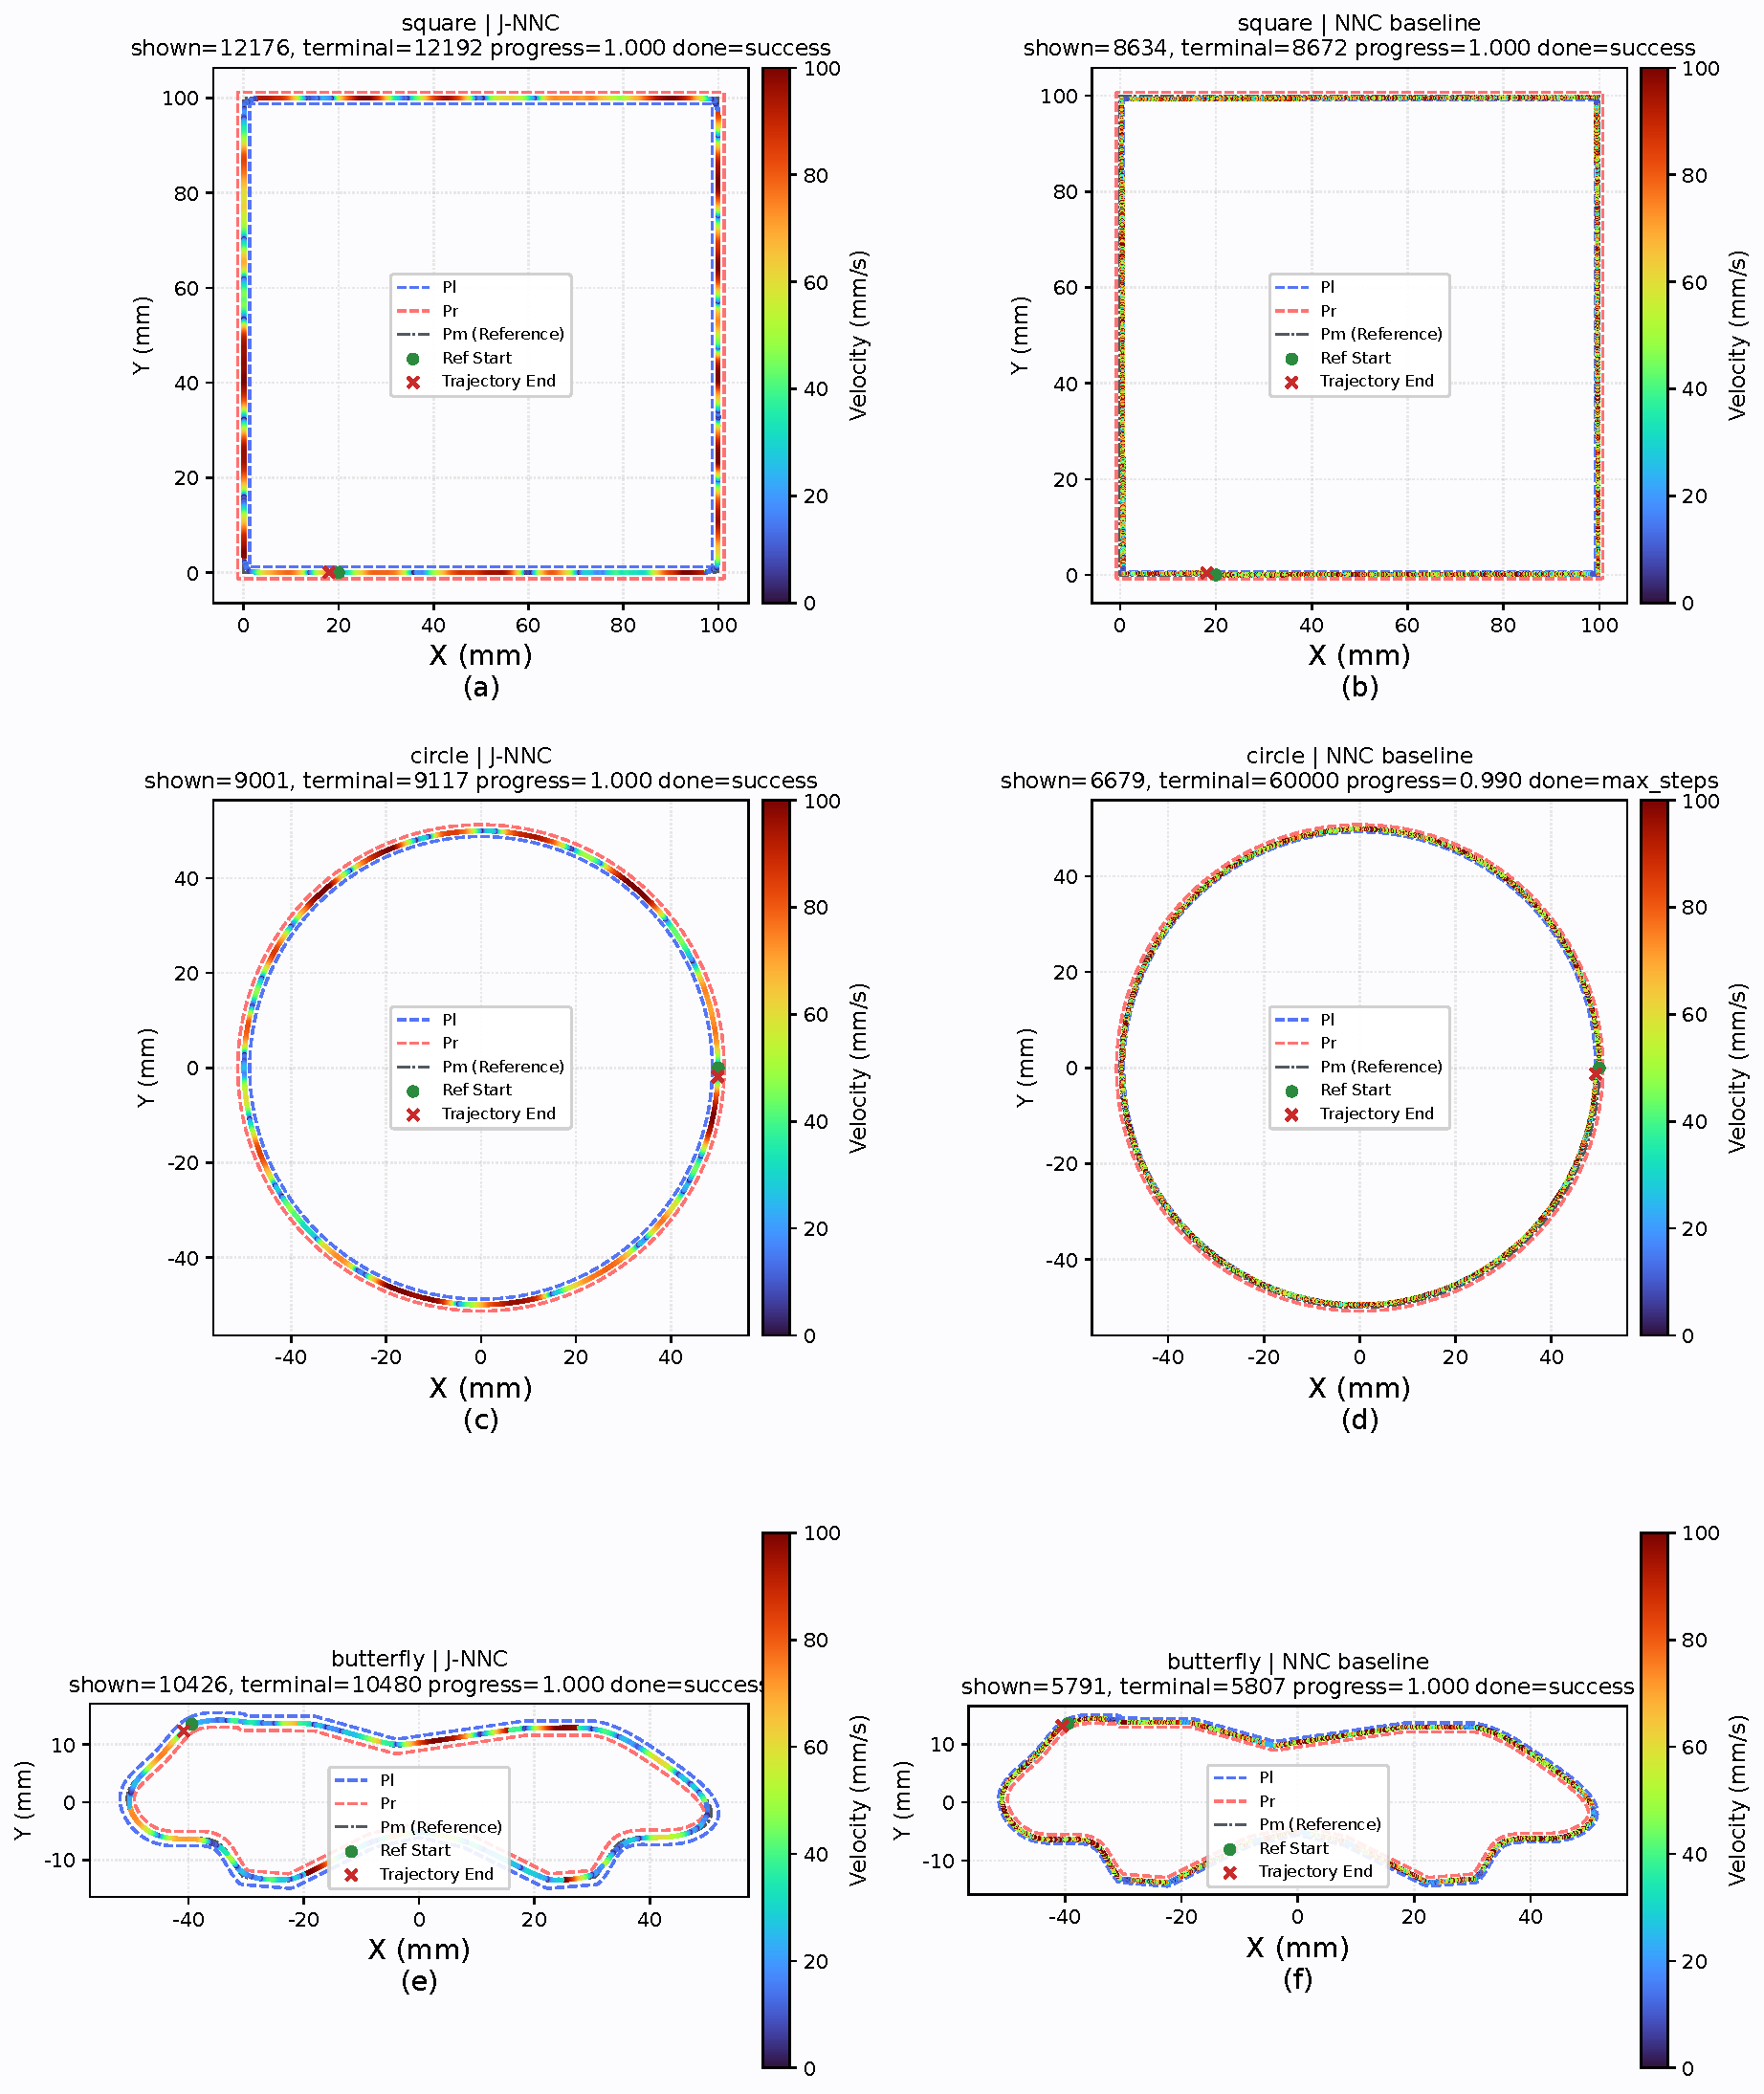
\includegraphics[width=0.96\linewidth]{figures/generated/qualitative_results.pdf}
        \caption{主方法与基线方法在代表性路径场景下的轨迹对比。}
        \label{fig:qualitative_results}
    \end{figure}
}{
    \begin{figure}[H]
        \centering
        \fbox{\parbox{0.9\linewidth}{\centering \vspace{2.8cm} 轨迹对比占位图：本文方法与基线方法在典型路径上的轨迹叠加、速度着色或局部放大图 \vspace{2.8cm}}}
        \caption{主方法与基线方法在典型路径场景下的轨迹对比。}
        \label{fig:qualitative_results}
    \end{figure}
}

图~\ref{fig:qualitative_results}中，本文方法生成的轨迹位于允差带内，并没有完全贴合参考折线。圆形路径中，本文方法的轨迹连续推进，速度变化较平稳。正方形路径中，本文方法在角点附近形成局部过渡。蝴蝶形路径中，本文方法在曲率变化区域产生一定偏移。上述现象说明，本文方法利用允差带进行局部轨迹调整，以减小拐角或曲率变化处的控制量突变。

正方形路径的拐角区域对比见图~\ref{fig:square_corner_zoom}。

\IfFileExists{figures/generated/square_corner_zoom.pdf}{
    \begin{figure}[H]
        \centering
        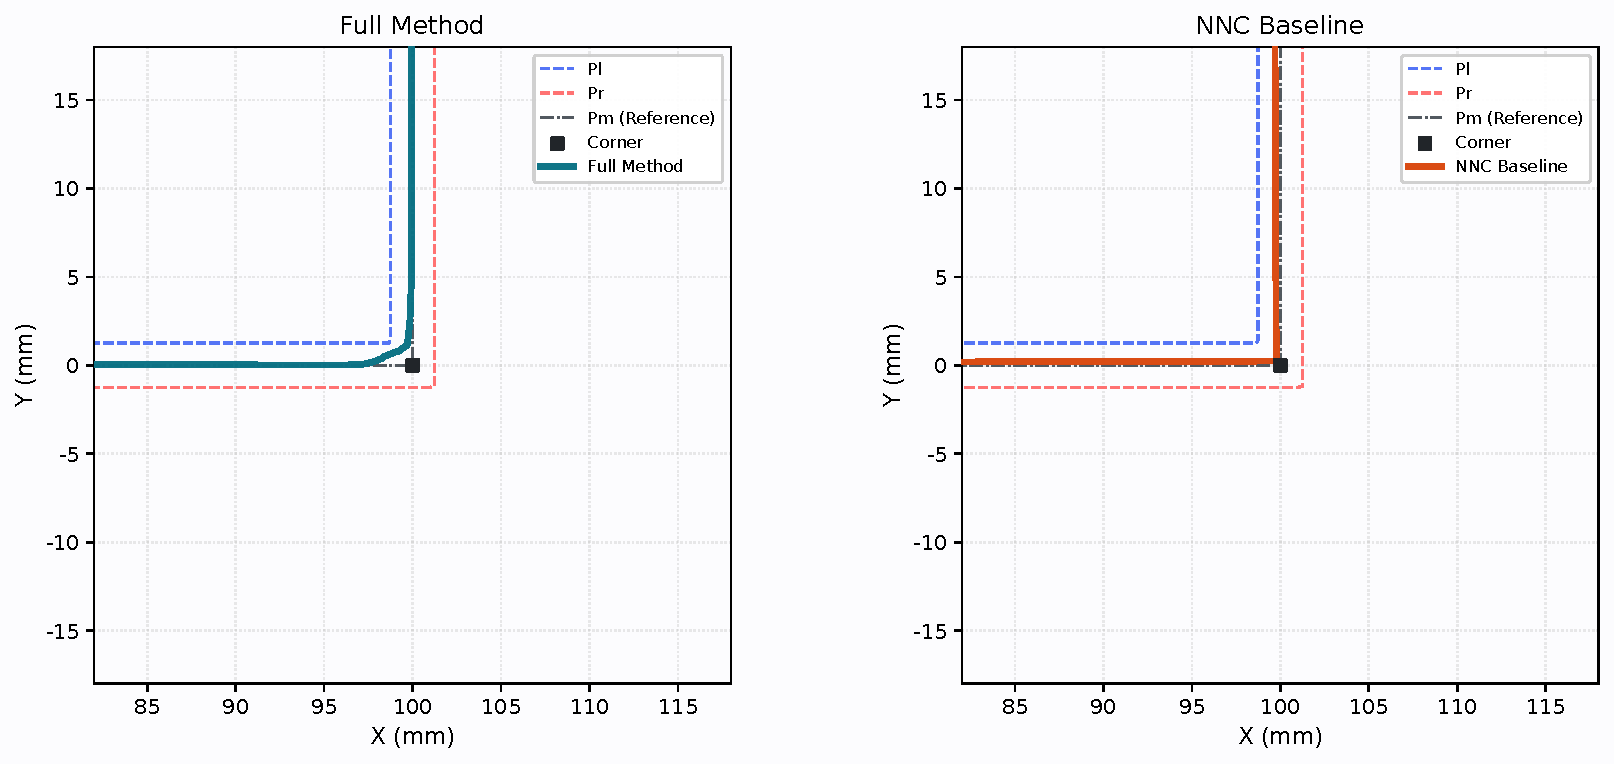
\includegraphics[width=0.92\linewidth]{figures/generated/square_corner_zoom.pdf}
        \caption{主方法与 NNC 方法在正方形路径拐角区域的局部放大轨迹对比。}
        \label{fig:square_corner_zoom}
    \end{figure}
}{
    \begin{figure}[H]
        \centering
        \fbox{\parbox{0.9\linewidth}{\centering \vspace{2.8cm} 正方形拐角局部放大占位图：主方法与基线在同一角点附近的局部轨迹高清对比 \vspace{2.8cm}}}
        \caption{主方法与 NNC 方法在正方形路径拐角区域的局部放大轨迹对比。}
        \label{fig:square_corner_zoom}
    \end{figure}
}

图~\ref{fig:square_corner_zoom}显示，本文方法在接近角点前开始改变方向，在允差带内形成连续过渡轨迹。NNC 方法的轨迹更接近原始折线，方向变化集中在拐角点附近。该现象与表~\ref{tab:main_results}中的捷度结果一致。直接执行策略输出时，拐角处容易出现较大的动态变化；经过 KCM 约束后，本文方法能够在转向过程中满足捷度限制。

本文方法在代表性 best rollout 上的轮廓误差、速度与线捷度归一化时序如图~\ref{fig:kcm_analysis}所示。

\IfFileExists{figures/generated/kcm_analysis.pdf}{
    \begin{figure}[H]
        \centering
        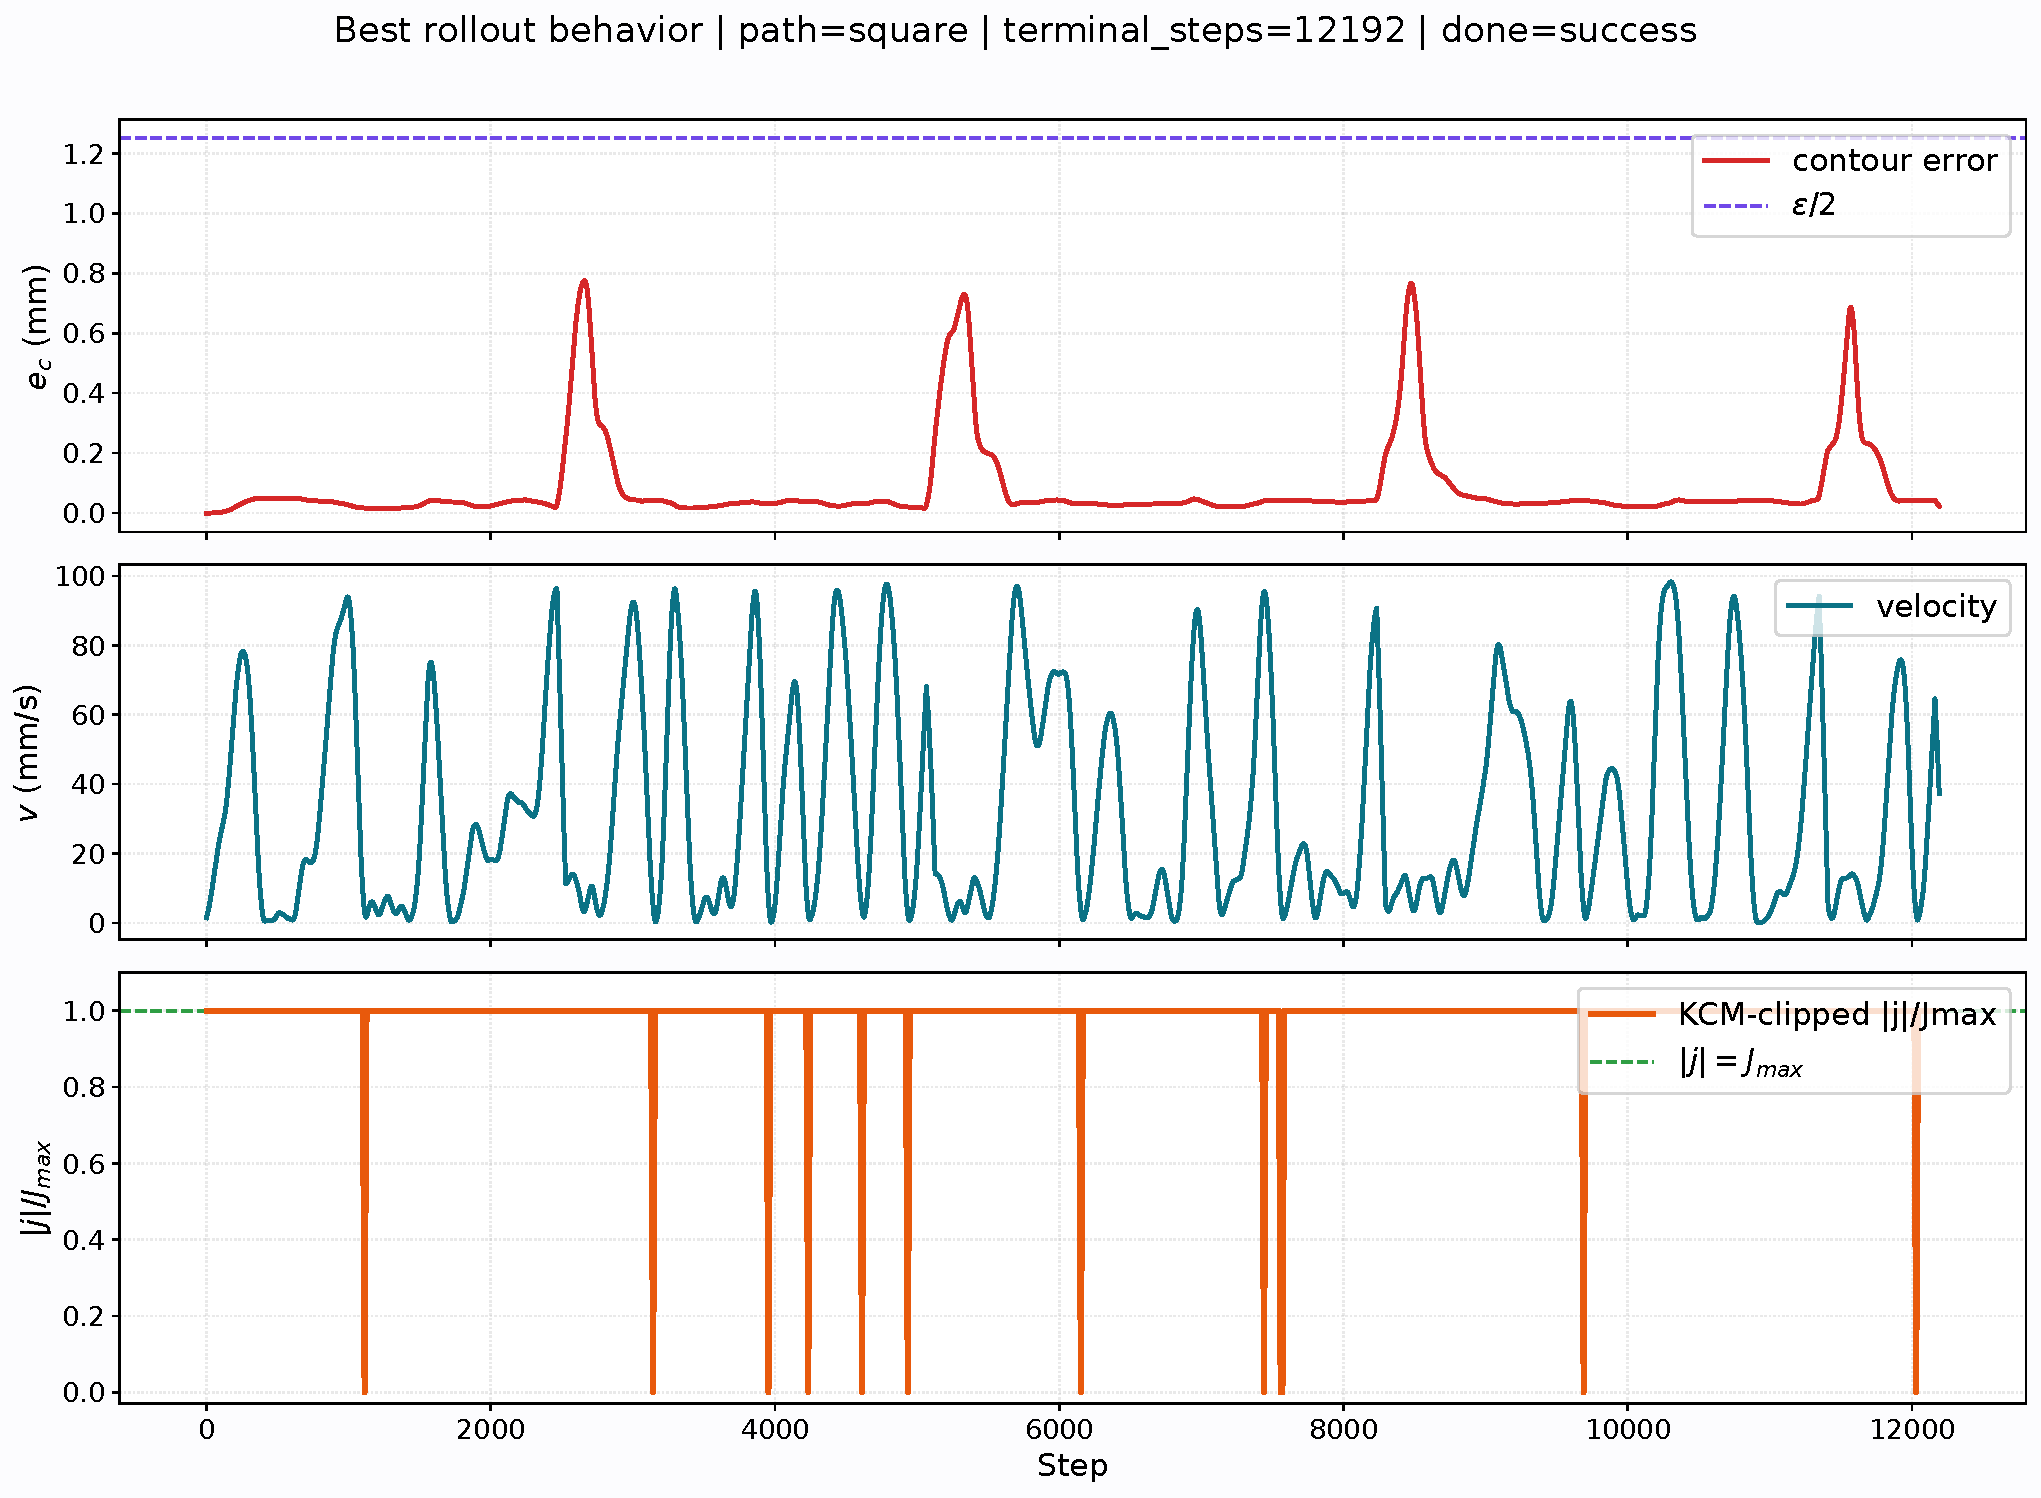
\includegraphics[width=0.96\linewidth]{figures/generated/kcm_analysis.pdf}
        \caption{本文最终方法在选定代表性 best rollout 上的轮廓误差、速度与线捷度归一化时序。}
        \label{fig:kcm_analysis}
    \end{figure}
}{
    \begin{figure}[H]
        \centering
        \fbox{\parbox{0.9\linewidth}{\centering \vspace{2.8cm} 行为解释占位图：前瞻距离、KCM干预度、误差和速度在拐角区的时序对齐图 \vspace{2.8cm}}}
        \caption{前瞻调节、KCM干预度与拐角行为解释图。}
        \label{fig:kcm_analysis}
    \end{figure}
}

图~\ref{fig:kcm_analysis}中，轮廓误差峰值主要出现在拐角阶段，说明策略在过弯时使用了允差带中的空间。速度曲线反映了进入拐角、通过拐角和离开拐角时的调速过程。当前历史 best rollout 的轨迹 CSV 未直接保存环境内部逐步捷度字段，因此图中给出由同一 best rollout 的速度记录经 KCM 边界复核得到的窗口峰值 $|j|/J_{\max}$ 曲线；该曲线不超过 1，结合表~\ref{tab:main_results}可知，启用 KCM 后线捷度最大相对超限为零。

综合表~\ref{tab:main_results}与图~\ref{fig:qualitative_results}至图~\ref{fig:kcm_analysis}可以看出，本文方法在三类路径上均完成 best rollout，并能够在直线高速进给和拐角处的允差带内形成局部平滑轨迹。对于正方形尖角和蝴蝶形混合曲率区域，本文方法通过适当的轨迹平滑和 KCM 约束，使拐角或曲率变化处的执行控制量保持在运动学边界内。NNC 方法体现出直接神经控制的推进能力，但缺少显式约束处理时，不具备动态可执行性。

\subsection{消融实验结果}

本小节给出可学习前瞻距离、KCM、前瞻观测以及直线/拐角双奖励等模块的消融结果。表~\ref{tab:ablation}按路径汇总不同配置 best rollout 的终止状态、最终进度、最大轮廓误差、线捷度最大相对超限和终止时间。

\IfFileExists{generated/ablation_table.tex}{
    \begin{table}[H]
\centering
\caption{Path-level results of the structured ablation study.}
\label{tab:ablation}
\begingroup
\small
\setlength{\tabcolsep}{3pt}
\renewcommand{\arraystretch}{1.16}
\resizebox{0.98\textwidth}{!}{%
\begin{tabular}{>{\raggedright\arraybackslash}p{0.23\textwidth}lccccc}
\toprule
\textbf{Configuration} & \textbf{Path} & \textbf{Outcome} & \textbf{Final progress} & \begin{tabular}[c]{@{}c@{}}\textbf{Peak contour}\\\textbf{error [mm]}\end{tabular} & \begin{tabular}[c]{@{}c@{}}\textbf{Peak jerk-limit}\\\textbf{exceedance}\end{tabular} & \textbf{Elapsed time [s]}\\
\midrule
\multirow{3}{0.23\textwidth}{J-NNC} & square & success & 1.000 & 0.834 & 0.000 & 12.192\\
& circle & success & 1.000 & 0.096 & 0.000 & 9.117\\
& butterfly & success & 1.000 & 0.745 & 0.000 & 10.480\\
\addlinespace[0.35em]
\multirow{3}{0.23\textwidth}{Fixed Adaptive Preview} & square & success & 1.000 & 0.699 & 0.000 & 8.680\\
& circle & success & 1.000 & 0.046 & 0.000 & 4.804\\
& butterfly & success & 1.000 & 0.638 & 0.000 & 5.049\\
\addlinespace[0.35em]
\multirow{3}{0.23\textwidth}{Without KCM} & square & success & 1.000 & 0.722 & 3199.000 & 10.301\\
& circle & success & 1.000 & 0.061 & 3199.000 & 5.926\\
& butterfly & success & 1.000 & 0.707 & 3199.000 & 7.446\\
\addlinespace[0.35em]
\multirow{3}{0.23\textwidth}{Without Adaptive Preview observation} & square & success & 1.000 & 0.805 & 0.000 & 8.151\\
& circle & success & 1.000 & 0.077 & 0.000 & 4.573\\
& butterfly & success & 1.000 & 0.820 & 0.000 & 6.044\\
\addlinespace[0.35em]
\multirow{3}{0.23\textwidth}{Without straight-line/corner dual rewards} & square & success & 1.000 & 0.824 & 0.000 & 15.132\\
& circle & success & 1.000 & 0.030 & 0.000 & 10.388\\
& butterfly & success & 1.000 & 0.918 & 0.000 & 9.623\\
\bottomrule
\end{tabular}
}
\endgroup
\end{table}

}{
    \begin{table}[H]
    \centering
    \caption{结构化消融路径级结果汇总。}
    \label{tab:ablation}
    \begin{tabular}{llccccc}
    \toprule
    \textbf{模型配置} & \textbf{路径} & \textbf{终止状态} & \textbf{最终进度} & \textbf{最大轮廓误差} & \textbf{线捷度最大相对超限} & \textbf{终止时间 (s)}\\
    \midrule
    本文最终方法 & square & 待填 & 待填 & 待填 & 待填 & 待填\\
    本文最终方法 & circle & 待填 & 待填 & 待填 & 待填 & 待填\\
    本文最终方法 & butterfly & 待填 & 待填 & 待填 & 待填 & 待填\\
    固定前瞻 & square & 待填 & 待填 & 待填 & 待填 & 待填\\
    固定前瞻 & circle & 待填 & 待填 & 待填 & 待填 & 待填\\
    固定前瞻 & butterfly & 待填 & 待填 & 待填 & 待填 & 待填\\
    无KCM & square & 待填 & 待填 & 待填 & 待填 & 待填\\
    无KCM & circle & 待填 & 待填 & 待填 & 待填 & 待填\\
    无KCM & butterfly & 待填 & 待填 & 待填 & 待填 & 待填\\
    无前瞻观测 & square & 待填 & 待填 & 待填 & 待填 & 待填\\
    无前瞻观测 & circle & 待填 & 待填 & 待填 & 待填 & 待填\\
    无前瞻观测 & butterfly & 待填 & 待填 & 待填 & 待填 & 待填\\
    无直线/拐角双奖励 & square & 待填 & 待填 & 待填 & 待填 & 待填\\
    无直线/拐角双奖励 & circle & 待填 & 待填 & 待填 & 待填 & 待填\\
    无直线/拐角双奖励 & butterfly & 待填 & 待填 & 待填 & 待填 & 待填\\
    \bottomrule
    \end{tabular}
    \end{table}
}

表~\ref{tab:ablation}显示，各消融配置在三条路径的 best rollout 上均能成功终止，但终止时间、轮廓误差和捷度约束满足情况存在差异。固定前瞻配置反映了前瞻距离在线调节的影响，无前瞻观测配置反映了多尺度几何信息的影响，无直线/拐角双奖励配置反映了阶段化奖励调度的影响，无 KCM 配置用于分析执行层约束投影的作用。除无 KCM 配置外，其余配置均启用 KCM，因此线捷度最大相对超限为零。

本文最终方法与无 KCM 配置在相同代表性路径上的线捷度对比如图~\ref{fig:jerk_constraint_comparison}所示。

\IfFileExists{figures/generated/jerk_constraint_comparison.pdf}{
    \begin{figure}[H]
        \centering
        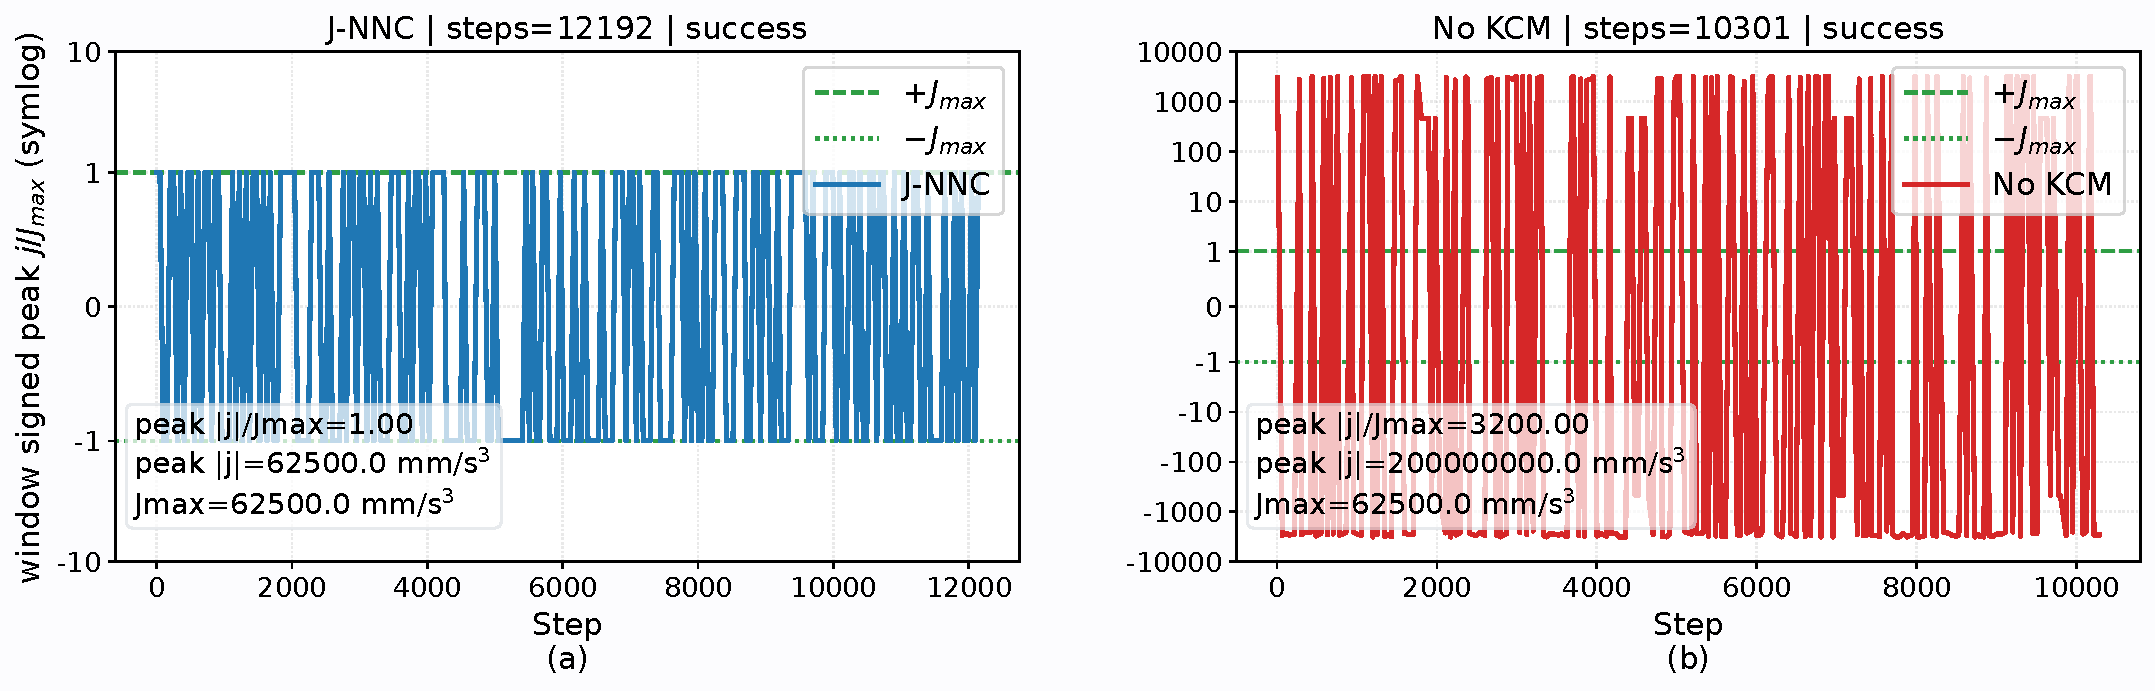
\includegraphics[width=0.96\linewidth]{figures/generated/jerk_constraint_comparison.pdf}
        \caption{本文最终方法与无 KCM 消融在相同代表性路径上的线捷度与捷度约束对比。}
        \label{fig:jerk_constraint_comparison}
    \end{figure}
}{
    \begin{figure}[H]
        \centering
        \fbox{\parbox{0.9\linewidth}{\centering \vspace{2.8cm} 捷度约束对比占位图：本文最终方法与无KCM消融在相同路径上的线捷度及其约束上界对比 \vspace{2.8cm}}}
        \caption{本文最终方法与无 KCM 消融在相同代表性路径上的线捷度与捷度约束对比。}
        \label{fig:jerk_constraint_comparison}
    \end{figure}
}

图~\ref{fig:jerk_constraint_comparison}显示，本文最终方法的线捷度被限制在 $J_{\max}$ 边界内，无 KCM 配置在相同路径上出现高幅值捷度尖峰。该结果说明，用时较短或轮廓误差较小并不一定代表轨迹可执行。KCM 对本文方法是必要模块，其作用是将策略输出转化为满足速度、加速度与捷度约束的执行控制量。

固定前瞻配置用于观察前瞻距离调节分量的作用。该配置保留前方几何感知结构，采用固定前瞻长度进行决策。结合表~\ref{tab:ablation}可见，固定前瞻在三条路径上均成功终止，且部分路径终止时间较短。可学习前瞻距离为策略提供了在线调节感知尺度的自由度，同时也增加了动作空间维度，其效果与路径复杂度、奖励权重和 KCM 干预程度相关。当前结果说明，前瞻距离动作的参数化方式仍需要进一步调整，使其更稳定地服务于提前调速和拐角预处理，而不能仅以终止时间单项判断其作用。

无前瞻观测配置用于观察多尺度前方几何信息的作用。该配置保留可学习前瞻距离和 KCM 约束执行，移除多尺度前瞻观测状态。结合表~\ref{tab:ablation}可见，局部状态和拐角感知能够支撑三条路径的基本推进，但不同路径上的终止时间和轮廓误差发生变化。多尺度前瞻观测为策略提供更完整的前方几何趋势信息，主要作用于复杂混合路径中的提前减速、提前转向和速度衔接。该模块的收益需要在更长路径、更密集拐角和更复杂曲率变化中进一步验证。

无直线/拐角双奖励配置用于考察阶段化奖励的作用。该配置采用统一奖励权重处理直线进给、进入拐角、过弯和离开阶段。结合表~\ref{tab:ablation}可见，移除该模块后跨路径完成稳定性下降。直线段主要要求稳定进给和方向一致，拐角段主要要求控制误差、降低速度变化并平滑转向。如果所有阶段使用同一奖励权重，策略在直线段和拐角段之间切换时更容易出现不稳定行为。因此，直线/拐角双奖励能够使策略在不同几何阶段采用不同的控制方式。

综合表~\ref{tab:ablation}与图~\ref{fig:jerk_constraint_comparison}可以看出，KCM 主要保证执行轨迹的动态可行性，直线/拐角双奖励主要影响不同几何阶段的行为稳定性，可学习前瞻距离与多尺度前瞻观测主要提供前方几何感知与在线调节能力。当前结果同时表明，square 闭合路径虽然能够成功终止，但终止时间和拐角后速度衔接仍是影响实验效率的重要因素，需要在后续优化中单独处理。

\subsection{本节小结}

主对照实验表明，本文方法在三条代表性路径上均能够形成有效轨迹，并且能够将执行控制量限制在给定运动学边界内。与 NNC 方法相比，本文方法的主要优势是动态可执行性更强，在拐角和曲率变化区域能够避免捷度超限。

消融实验表明，KCM 是保证约束满足的关键模块，直线/拐角双奖励有助于提高跨路径稳定性。可学习前瞻距离和多尺度前瞻观测提供了几何感知和在线调节能力。总体来看，本文方法能够在保持路径推进的同时满足运动学约束，适合用于强调动态可执行性的数控运动规划场景。

\section{局限性分析与未来展望}
\label{sec:conclusion}

本文方法仍有若干不足。首先，可学习前瞻距离虽然增加了在线调节自由度，但在当前实验中，其优势尚未稳定转化为更短用时，说明前瞻距离分量的参数化方式仍需改进。其次，方法在不同几何路径上的表现还不完全均衡。对于连续曲率路径，策略较容易形成稳定的速度调节；对于含尖角或混合曲率变化的路径，阶段切换、终点收敛和局部过弯仍是主要难点。最后，KCM 能够保证执行控制量满足运动学约束，但也可能带来更保守的速度变化，说明策略本体尚需进一步学习贴合约束边界的控制规律。

后续工作将从三方面展开。第一，改进动作空间中前瞻距离分量的参数化方式，例如采用残差式、分段式或与拐角相位相关的前瞻参数化，以降低学习难度并减少与前瞻观测之间的冗余。第二，细化拐角阶段建模，重点处理尖角进入、过弯、离开和终点停止等局部过程，提高复杂路径下的完成率与速度衔接稳定性。第三，扩大测试路径集合，并进一步引入伺服滞后、轴向约束和实机加工条件，使仿真中的允差带利用、时间效率和捷度约束评价逐步接近实际 CNC 运动规划需求。

\clearpage
\phantomsection
\section*{附录}
\addcontentsline{toc}{section}{附录}

\subsection*{PPO 训练设置}
策略采用 Proximal Policy Optimization。Actor 为三层共享多层感知机，隐藏层宽度依次为 $256,128,64$，激活函数为 ELU，每层后使用 LayerNorm，输出头给出 3 维动作的均值和标准差；其中转向动作均值经 $\tanh$ 限制到 $[-1,1]$，进给和前瞻动作均值经 sigmoid 限制到 $[0,1]$，标准差经 softplus 后加 $10^{-3}$。Critic 为 $256,128,64,1$ 结构，使用 ELU、LayerNorm 和 $0.1$ dropout。

\begin{table}[H]
\centering
\caption{PPO 超参数与训练协议。}
\label{tab:appendix_ppo_params}
\small
\begin{tabular}{lp{0.68\textwidth}}
\toprule
\textbf{参数} & \textbf{取值}\\
\midrule
Actor 学习率 & $3.0\times10^{-4}$\\
Critic 学习率 & $1.5\times10^{-4}$\\
折扣因子 $\gamma$ & $0.99$\\
GAE 参数 $\lambda$ & $0.95$\\
PPO clip 系数 & $0.1$\\
每次更新 epoch 数 & $8$\\
熵系数 & $0.01$\\
梯度裁剪 & $0.5$\\

\bottomrule
\end{tabular}
\end{table}

\subsection*{KCM约束投影算法}

\begin{algorithm}[H]
\caption{KCM约束投影过程}
\label{alg:kcm}
\begin{algorithmic}[1]
\Require 策略输出 $a_t^{\pi}=[u_{\theta,t},u_{v,t},u_{L,t}]$；上一时刻运动学状态 $(v_{t-1},a_{t-1},\omega_{t-1},\alpha_{t-1})$
\Ensure 执行控制量 $(\omega_t,v_t)$ 及更新后的运动学状态
\State 将 $u_{\theta,t}$ 与 $u_{v,t}$ 映射为约束前运动控制量 $(\omega_t^{pre},v_t^{pre})$
\State 将 $u_{L,t}$ 映射为当前前瞻距离 $L_t$
\State 根据 $v_t^{pre}$ 与 $v_{t-1}$ 计算约束前线加速度 $a_t^{pre}$
\State 根据 $a_t^{pre}$ 与 $a_{t-1}$ 计算约束前线捷度 $j_t^{pre}$
\State 对 $j_t^{pre}$ 进行裁剪，得到满足上限的 $j_t$
\State 由 $j_t$ 反算线加速度 $a_t$，并执行加速度裁剪
\State 由 $(v_{t-1},a_{t-1},j_t)$ 积分得到本周期线速度 $v_t$
\State 对角速度通道采用同构流程，得到约束后的 $\omega_t$
\State 返回执行控制量 $(\omega_t,v_t)$ 及相应更新后的运动学状态
\end{algorithmic}
\end{algorithm}

\clearpage
\bibliographystyle{unsrt}
\bibliography{references}

\end{document}
